\chapter{Results}
ergebnisse (screenshots \/ source code)

\section{Draw Sphere Cells}
\begin{figure}
	\center
	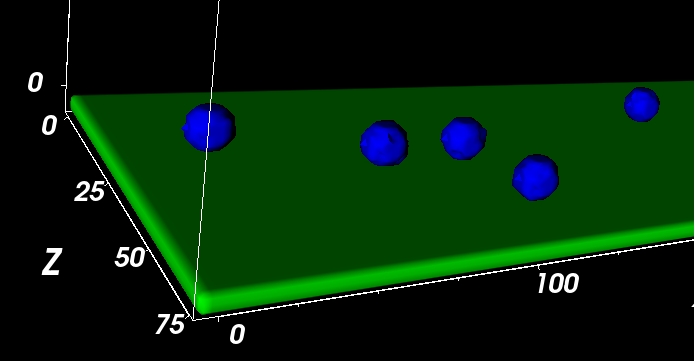
\includegraphics[scale=0.6]{figures/DrawnSphereCell.png}
	\caption{A cell drawn as a sphere}
	\label{img:DrawnSphereCell}
\end{figure}
With the created method the program is now able to draw a sphere. Since we use voxels in the 3D simulation, it is not possible to draw a round sphere. Thus, an approximation to the volume, surface and the shape has to be done with these voxels. This approximation to a real sphere allows us to draw cells, which look like spheres, and also let them growth with their shape. Since in the simulation are lattice constraints as well as other cells, it is possible that the shape of a sphere will not be kept during the simulation. Moreover, the deviation of the volume and surface between the in pixels drawn and grown sphere to a real sphere grows \textbf{expontially} as the radius of the sphere grows as it is displayed in \textbf{figure XY}.
A result of a drawn cell with different radius and voxel densities is displayed at \textbf{figure xy}.


A factor the approximation to an real sphere is the voxel density. It describes how many voxel display \SI{1}{\micro\metre}. As an example, if the voxel density = 1 than it represents \SI{1}{\micro\metre}, if the voxel density = 2 than one voxel represents \SI{0.5}{\micro\metre} and so on. In a simulation with \SI{100}{\micro\metre} at the x-axis, \SI{80}{\micro\metre} at the y-axis and \SI{50}{\micro\metre} at the z-axis is displayed with 100 voxel at the x-axis, 80 voxel at the y-axis and 50 voxel at the z-axis for a voxel density of 1. With a voxel density of 2 the lattice of the simulation would include 200 voxel at the x-axis, 160 voxel at the y-axis and 100 voxel at the z-axis. Thus, the radius of a cell is also dependend of the voxel density. Considering that the radius growths as the voxel density growths and that between the calculated sphere, out of pixels, and a real sphere the deviation growths further apart as the radius growths it is not correct to say that with a higher voxel density there will be a more accurate result. Because, the approximation error is larger for voxel density of 2 it is possible that the approximation errors effects the accuracity of the simulation in a negative way. This fact has to be checked in a future work.